\section{Results}
We can now look into the results of our work and show how we can create our different variations of the game. As we have already discussed, we can give the player three different abilities and likewise we can give the boss two different abilities, but we can also choose not to have a boss. The room can take a combination of four weathers, and based on those, we can meet different weather effects in the game variations. We can thus create \textbf{36} different variations.

\begin{figure}[H]
	\centering
	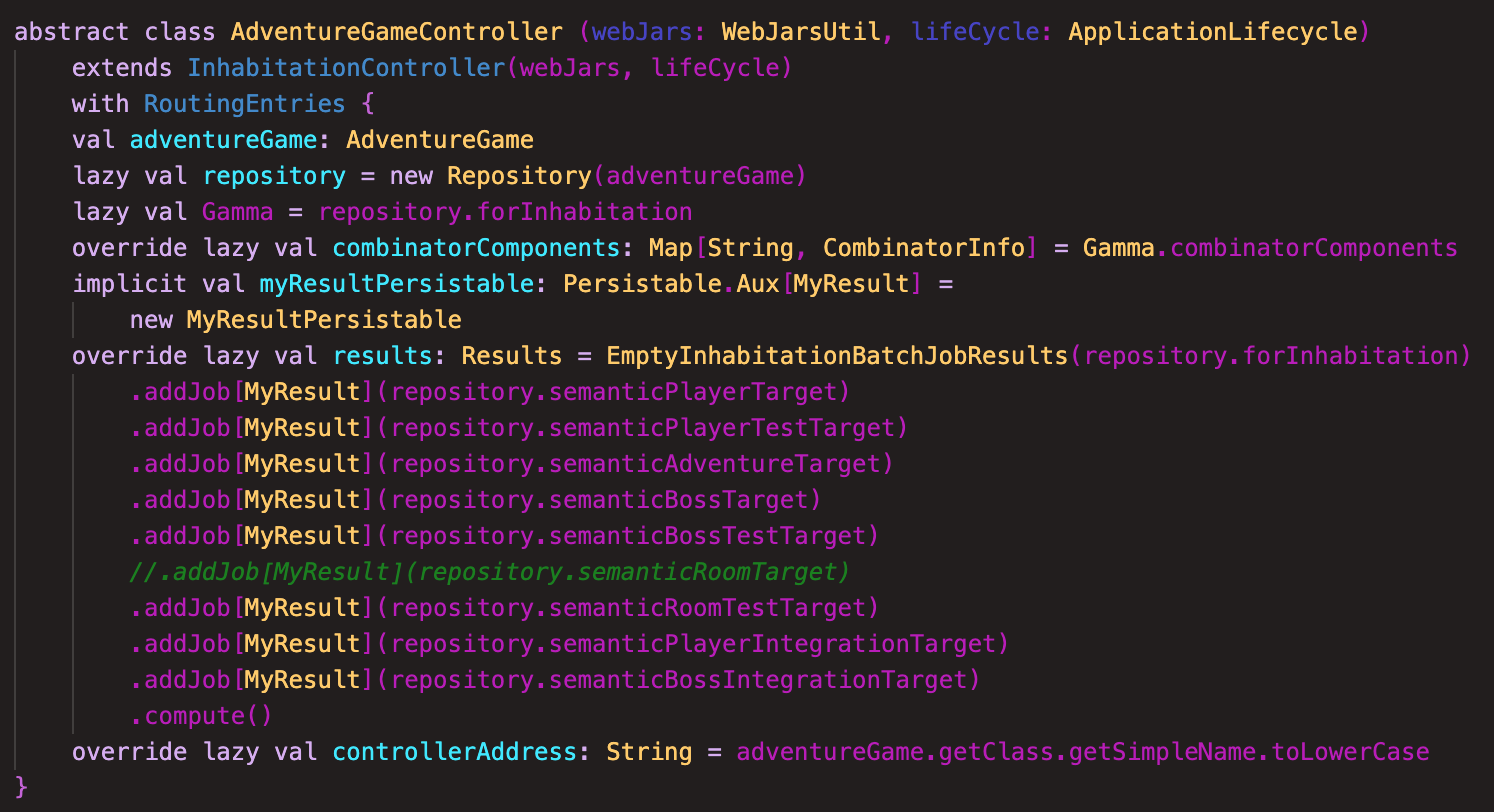
\includegraphics[width=\linewidth]{Materials/Results/AdventureController}
	\caption{In the \textit{AdventureGameController} we can see what jobs we are scheduling and thus what we want synthesized.}
	\label{Controller}
\end{figure}
In \autoref{Controller} we see \textit{AdventureGameController} in which we add the jobs we want done. Each job correspond to a synthesis we want done, and so if we are only interested in creating a player we could remove the other jobs.

\begin{figure}[H]
	\centering
	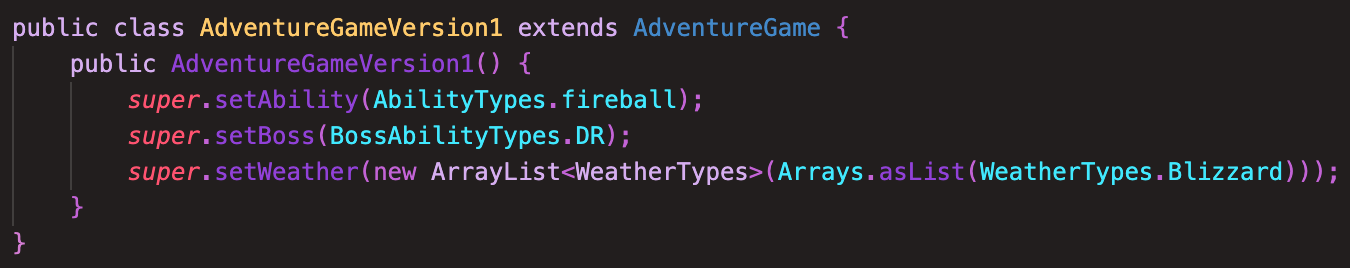
\includegraphics[width=\linewidth]{Materials/Results/AdventureVariation}
	\caption{By setting the \textit{AdventureGame} fields we can create different variation of our game. Here is shown a variation where the player has the fireball, the boss has the damage reduction ability and the possible weather effects would be blizzard.}
	\label{version1}
\end{figure}

To alter the variation we synthesize we need to look at a concrete class which extends our \textit{AdventureGame} class. We can here look at \textit{AdventureGameVersion1} which is seen in \autoref{version1}. We here see the player having the fireball ability, the boss having the damage reduction ability, and the possible weather effects being blizzard.

\begin{wrapfigure}{R}{0.6\linewidth}
	\centering
	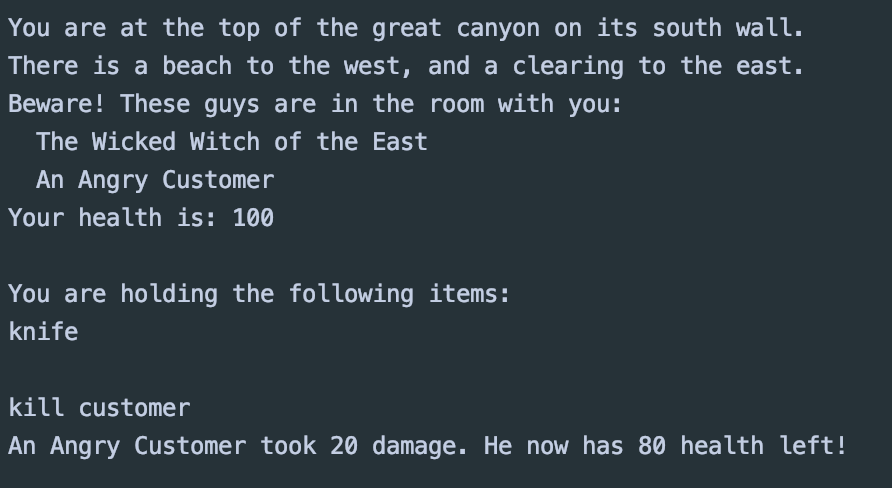
\includegraphics[width=\linewidth]{Materials/Results/AttackingCustomer}
	\caption{We see that the player with the knife can attack the Angry Customer.}
	\label{sc1}
\end{wrapfigure}
In the following we will showcase that the initial application can be synthesized and played. Here we are focusing on \autoref{sc1}, \autoref{sc2} and \autoref{sc3}. As we start the game we see that we can not hit other players in the room with us. This is because we need the knife to attack with, as we do not have the fireball in the initial application. With the knife we can now begin stabbing both other players, but also the evil customer monster. The concept for hitting the 'Wicked Witch' is the same, but here we need the water. As this is all there is to the game in the initial application, our showcase of the initial application is done.

\begin{figure}[H]
	\centering
	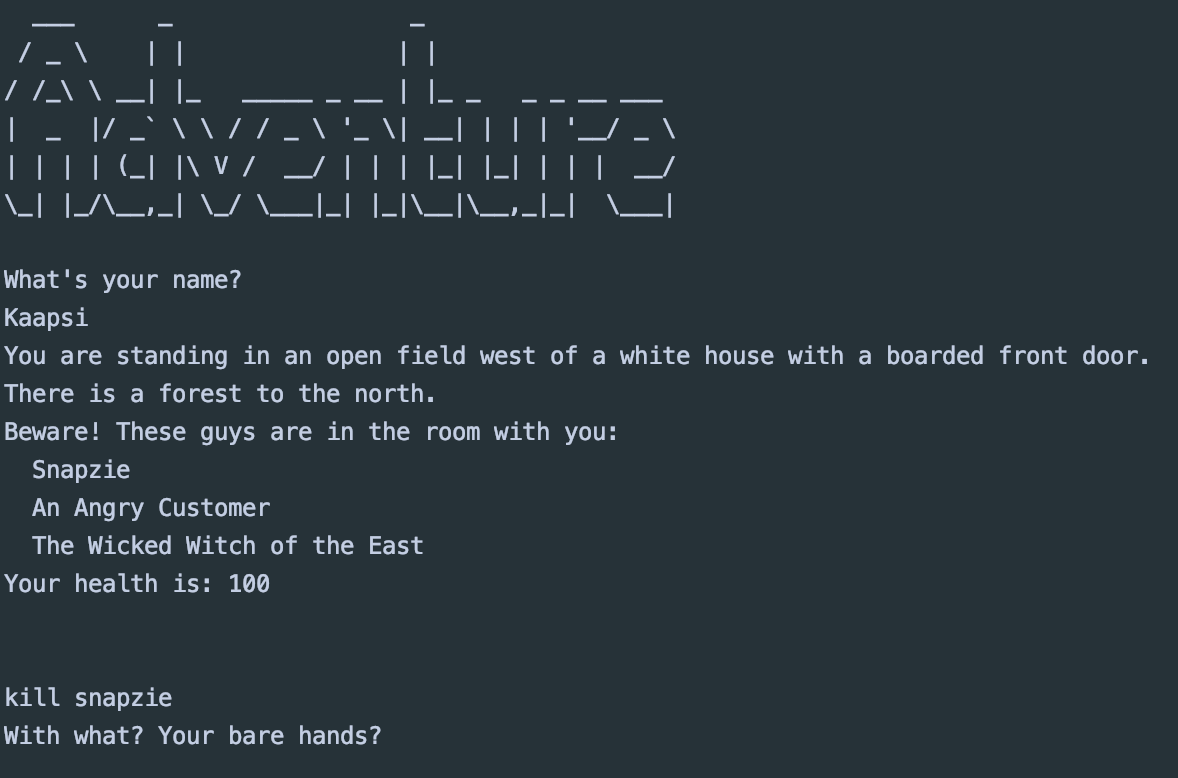
\includegraphics[width=0.9\linewidth]{Materials/Results/PlayersEntering}
	\caption{We see that we cannot attack other players without having the knife.}
	\label{sc2}
\end{figure}

\begin{figure}[H]
	\centering
	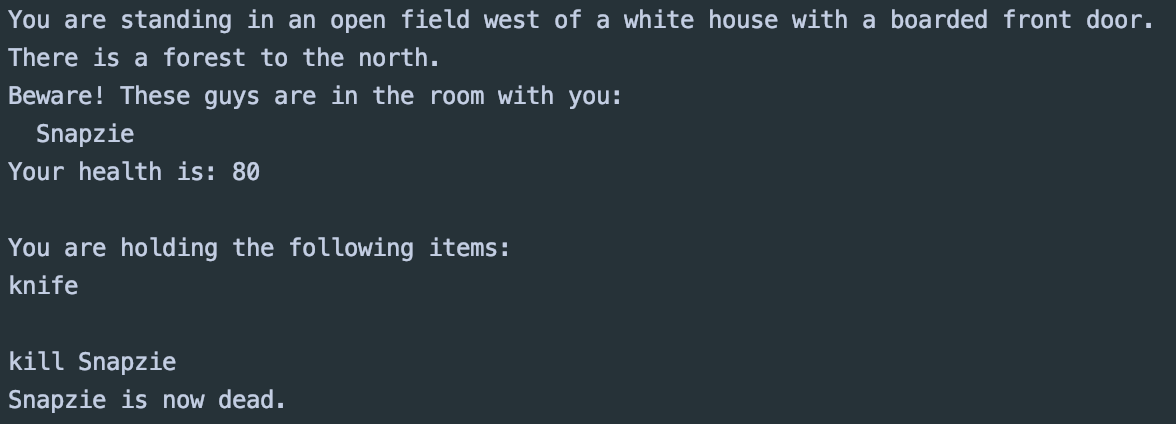
\includegraphics[width=0.8\linewidth]{Materials/Results/AttackingPlayer}
	\caption{We see that the player with the knife can attack other players.}
	\label{sc3}
\end{figure}

But to show off the weather effects and the boss, we have provided to more showcasing images for these variations, namely \autoref{sc4} and \autoref{sc5}.

\begin{figure}[H]
	\centering
	\includegraphics[width=0.6\linewidth]{example-image-a}
	\caption{We see that we cannot attack other players without having the knife.}
	\label{sc4}
\end{figure}

\begin{figure}[H]
	\centering
	\includegraphics[width=0.6\linewidth]{example-image-a}
	\caption{We see that the player with the knife can attack other players.}
	\label{sc5}
\end{figure}

\begin{wrapfigure}{L}{0.4\linewidth}
	\vspace{-10px}
	\centering
	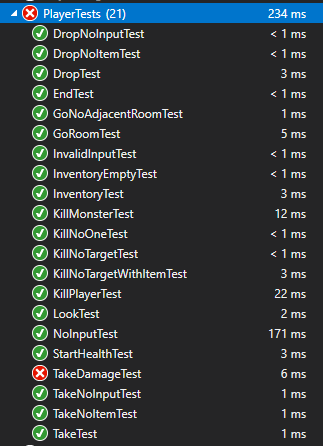
\includegraphics[width=\linewidth]{Materials/Results/PlayerUnitTestsInitial}
	\caption{A run of the tests, as they appear in the synthesized initial application.}
	\label{PlayerUnitInit}
\end{wrapfigure} 
Let us look at the results when it comes to testing. We have succeeded in creating the variations as explained above, including the corresponding tests. We add the tests as an individual job in the AdventureGameController. For instance, we can see in \autoref{Controller} how we both have a job for semanticPlayerTarget as well as semanticPlayerTestTarget. These are the player unit tests. \\
To test the initial application this way, we would need to synthesize it first. If we look at \autoref{version1}, we can set the different variables that create our variations of the game. In the case of the initial application, we would then have to set both setAbility and setBoss to their none types, as well as an empty setWeather\todo{ye?}.
In \autoref{PlayerUnitInit} we can see an example of one of the test suites run in the synthesized initial application, which is the player unit tests. These tests that appear in the initial application, without any variation will thus also appear in every variation of the game, meaning that variation only adds more tests. Earlier in the thesis, we have often referred to these as the essential tests because of this.
As we can see, all these tests succeeded, except the TakeDamage test. We went over why this test does not succeed in the subsection \nameref{getPrimaryKey}. We can also compare this figure to our table \autoref{tableTests} and see how, unsurprisingly, the initial application of course contains fewer player unit tests than in the table. This is because the table contains the total number of tests, meaning all of them across the different variations. With this, we have successfully synthesized and run the tests for the initial application. Again, this does mean that some of the tests cannot run, but as with TakeDamage, this is not due to any fault in synthesizing of the grains or tests, but rather a fault in the tests themselves. That is, the TakeDamage test, for instance, did not run before synthesizing it either. \\
It should also be mentioned that while we do not have a boss in the initial application, bossTests and bossIntegrationTests are still created, but they are empty, they do not contain any code or tests. This is due to the nature of combinators, where we combinate empty boss files when a boss is not present. \\
Now that we have seen the synthesizing of the initial application was a success, we can check other variations of the game and see how the tests react to this. For instance, if we keep the same setup as the initial application, but we apply the fireball to the player, we can see how the tests change. If we look at the player unit tests as we did with the initial application, we can see how this variation with fireball contains the same tests with new ones added. With this variation, all the fireball tests have been added except one. This is the FireballTestBoss, that was not combinated due to the boss not being present. If we compare the player fireball variation to our initial variation's player unit tests in \autoref{PlayerUnitInit}, we now have 25 tests instead of 21. 4 of our 5 fireball tests have thus been added, where the fifth as mentioned was the FireballTestBoss. Thus, we have been successful in synthesizing tests such that the correct tests are included in the different variations. %\\
%At last we should mention that while the synthesization was successful, we did not manage to make all the tests run, due to flaws in the our creation of them. However, while TakeDamageTest fails consistently, 
